\chapter{Discussion}

\begin{center}
    \textit{The results are analyzed and discussed in this chapter. It explores the implications of the findings, identifies limitations, and suggests potential areas for future improvement.}
\end{center}

\section{Temporary Title – Discussion of Results}

The model’s strategy of selecting the most likely move revealed a notable flaw in castling detection. Specifically, castling moves were often misclassified due to the system evaluating each piece movement independently. In many cases, the model assigned a higher confidence score to the rook's move from its original square than to the king’s two-square movement during castling. Consequently, 8 out of 9 misclassifications occurred when the model incorrectly selected the rook’s movement as the intended move, rather than recognizing the castling sequence. A possible solution is to briefly delay the rook’s movement, allowing the king’s two-square move to occur first. This removes ambiguity by ensuring that, at the moment of detection, only a single plausible move is visible—effectively forcing the model to select the castling move rather than misclassifying it as a standalone rook move. \\

Another recurring issue was observed in the form of consistent failure points within specific openings. In several test sets, all 10 games of a given opening failed at the same move number. This pattern suggests that certain positions or board states consistently challenge the model, possibly due to recurring piece configurations or lighting conditions at those points in the game. \\

Additionally, move detection accuracy decreased noticeably along the edges of the board. This limitation appears to result from a combination of factors. First, the board-warping algorithm relies on precise corner detection to accurately map square centers. While the inner squares were typically well-aligned, the outermost squares—particularly near the corners—were more prone to distortion, likely contributing to errors in piece localization. Second, the relatively steep camera angle made it harder to clearly distinguish pieces near the front edge of the board, as those closest to the lens were partially occluded or lacked visible detail. Third, pieces on the far side of the board appeared smaller in the frame, and the inter-square distances in the warped image were reduced. This made it more likely for pieces to be mistakenly assigned to adjacent squares, especially along the tighter edge regions. \\

Further testing supported these findings. As shown in Figure~\ref{fig:bbox-centers-incorrect}, the bounding boxes along the edges of the board are occasionally misaligned, reinforcing the challenges associated with edge square detection.

\begin{figure}[h!]
    \centering
    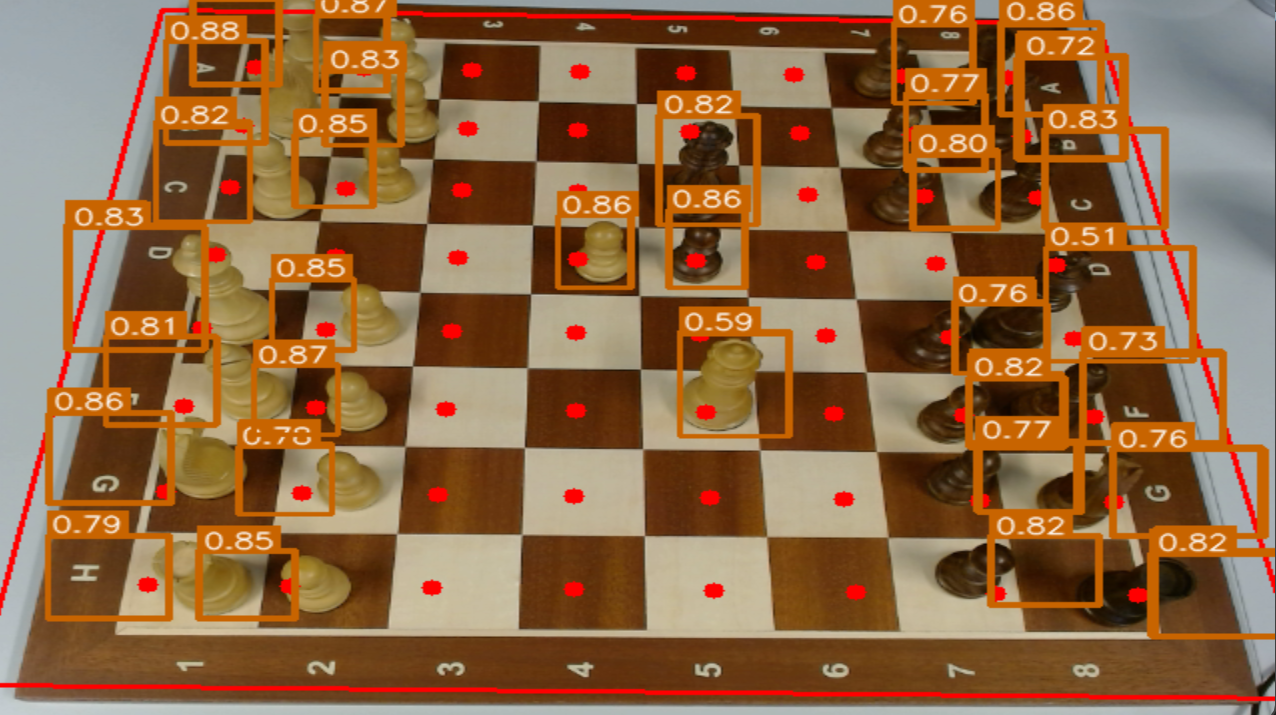
\includegraphics[width=0.75\linewidth]{figures/discussion/bbox-centers-incorrect.png}
    \caption{Bounding box centers overlaid on a physical chessboard. Some boxes near the edges are misaligned, indicating inaccuracies likely due to board edge detection, or model generalization limitations.}
    \label{fig:bbox-centers-incorrect}
\end{figure}



\subsubsection{Different gamemodes}

The models job is to find the pieces on the board and then assign them to its respective square. This means as long as you define the starting postion or start fen, that allows you to play any the game from any posistion you want. That means you could start a match mid game or you could play other game modes. The model also has validation so that means it should be able to successfully




\section{Further development}
Throughout the duration of this project, several ideas for development emerged. These from both the team, the product owner, and external contributors. Due to the time constraints of the Bachelor’s thesis, many of these ideas were not implemented and were therefore categorized as "Further development". After the product owner's request, ensuring accurate piece recognition was prioritized over extended functionality.

\subsection{Independent application}
Future plans include a standalone version of the application with ceiling-mounted cameras at the chess club. These would connect to a PC running the system continuously, operable via a physical switch. Players could set up boards and activate the system without technical knowledge. The application would start automatically, read boards in real time, and shut down via the same switch.

\subsection{Participant Management}
Players are currently hardcoded. A future version could allow manual registration through a UI, with data stored in a database. Integration with FIDE’s API could enable automatic rating retrieval.

\subsection{Time control}
The current system lacks time control tracking. Simple estimation based on timestamps is unreliable. Options include integrating digital clocks (costly) or using camera-based OCR to read physical clocks (technically complex and error-prone). This remains a future consideration. \\

\section{Obstacles}
In addition to ideas for future development, there were also a few obstacles encountered during the development phase of this project. These challenges were addressed as they occurred, and solutions were implemented as part of the final application.

\subsection{Camera}
During the development and testing phase of the front-end application, an obstacle related to camera initialization was encountered. The application is designed to access an external USB camera by specifying a camera ID other than 0, since ID 0 typically corresponds to the system's default or built-in (dashboard) camera, which is not relevant to this project.\\

Two identical external webcams were used for this project, both connected via a USB hub. One of the cameras functioned correctly. When connected, the front-end application successfully initialized the camera feed, and the video stream was displayed on the webpage as expected.\\

However, the second camera, did not behave as expected. Despite being physically identical to the first camera and verified to work through the system's built-in camera application, the front-end application failed to display its video feed. Instead, it defaulted to camera ID 0, resulting in the system's dashboard camera being selected.\\

This issue was traced back to a cached or “ghost” device entry in the Windows Device Manager. A ghost device refers to a previously connected hardware device that is no longer physically attached to the system but whose configuration and driver information remain cached by the operating system. These leftover entries can lead to conflicts or incorrect device indexing when similar hardware is reconnected, especially when multiple identical devices are used. In this case, the system appeared to retain prior camera associations, which caused the application to misidentify or incorrectly assign the camera index.

\subsection{Special moves}
When a move is made, the front-end highlights the previous and current tiles of the moved piece. User testing with different color palettes resulted in the selection of a bright contrast color relative to the main design scheme to ensure good visibility. \\

The chessboard component manages the rules of chess, while the front-end is responsible only for storing tile positions and applying styling. In standard moves, highlighting the starting and ending tiles is sufficient. However, special moves such as \gls{castling}, pawn \gls{promotion}, and \gls{en-passant} capture require additional handling. \\

In \gls{castling}, both the king and a rook move simultaneously. Since the default highlight logic tracks only one piece, it does not correctly represent \gls{castling} moves. Additional logic was implemented to highlight the movements of both the king and rook during \gls{castling}, ensuring consistency and clarity for the user.



\section{DELETED}

\section{Further development}
Throughout the duration of this project, several ideas for development emerged. These from both the team, the product owner, and external contributors. Due to the time constraints of the Bachelor’s thesis, many of these ideas were not implemented and were therefore categorized as "Further development". After the product owner's request, ensuring accurate piece recognition was prioritized over extended functionality.

\subsection{Independent application}
During the meeting with the product owner at Aalesund Schaklag's location, the product owner and the leader of the chess club discussed potential future developments. One idea was to implement a finished version of the application where cameras are permanently mounted on the ceiling at the club. Since the chess club typically maintains standard table arrangement for chessboards, the cameras would not need to be moved. \\

In this setup, the cameras would be connected to a computer located in a locked room, running the application continuously. The proposed solution involves connecting the system to a physical switch, enabling users to easily power the cameras and application on or off as needed. \\

A typical case would involve a group of chess players organizing a unofficial tournament. Upon arrival, the tables would already be positioned correctly under the cameras. The participants would set up their chessboards, pieces, and clocks, and then activate the system by turning on the switch. Once activated, the application would automatically start, and the cameras would begin reading the boards. Games would be tracked and displayed through the application in real time. Boards set back to their initial position would be recognized as reset. \\

After the tournament concludes, users could simply turn off the switch to shut down the system. This design enables the application to be used independently, without requiring technical expertise. It is intended to be accessible to both young adults and elderly users. Additionally, mounting the cameras on the ceiling contributes to enhanced security for the chess equipment.

\subsection{Information about participants}
In the current version of the application, all tournament participants are hardcoded directly into the code. This approach was chosen to allow the development team to focus on core functionality, particularly the accurate detection of board states. \\

A more flexible and maintainable solution would involve allowing the tournament organizer to manually register participants once tournament registration is complete. This could be implemented through a user interface, such as a form, with participant data stored in a database. Relevant information for each player would typically include their name, age, chess club affiliation, and chess rating. \\

One potential enhancement is to fetch player ratings directly from \gls{fide}, the international chess federation. \gls{fide} maintains the \gls{elo} rating system, which is the most widely used system for evaluating chess players and is also used by Aalesund Schaklag. When a player’s match is recorded in the \gls{fide} system, their rating is updated accordingly. By integrating with the \gls{fide} \gls{api} or database, the application could automatically retrieve up-to-date player ratings, ensuring accurate and consistent information for tournament use.

\subsection{Time control}
For spectators watching live chess games on a screen, it can be difficult to follow the pace of the game, as the current version of the application does not display any information about time control. Chess games are typically played with varying time formats, including \gls{classical}, \gls{blitz}, and \gls{bullet}, each of which allocates different amounts of time per player. Tournaments generally specify a single time control variant, which could be included in the tournament description. \\

A simple approach to improve spectator understanding would be to introduce a time control entity in the application. For example, if the tournament is set to use the \gls{blitz} format, the application could display an estimated countdown timer based on player moves. According to \gls{fide}, blitz games allocate 10 minutes or less per player. By knowing the variant in use, the application could estimate the time remaining based on the move timestamps. However, this method is not reliable, as several factors can introduce inaccuracies. This can be delays in move detection, move registration, and rendering on the screen. As a result, this solution would not provide precise or trustworthy time tracking. \\

An alternative is to use a digital chess clock, similar to those used with electronic chess boards. These clocks can be connected to a computer via cable and provide accurate time tracking. However, this method increases the cost of the setup significantly. A single digital clock can cost around 1,500 NOK, which goes against the application’s goal of being a low-cost and low-maintenance solution. \\

A more advanced approach would involve reading the clock visually using the same camera system that tracks the chessboard. In this solution, a machine learning model would be trained to recognize and interpret both the chessboard and the physical clock from the same image. The backend could then update the front-end with real-time clock values. While this approach would preserve the low-cost vision by removing the need for expensive clock hardware, it comes with technical challenges. The machine learning model could misread the clock due to obstructions, poor lighting, or low image resolution. For example, if a player’s hand is covering part of the clock, the system might not be able to detect the time correctly. These inaccuracies are particularly problematic in faster time formats like blitz or bullet, where even small errors or delays can significantly affect the perceived game state. \\

Due to these limitations and the project's scope, implementing time control features was not prioritized in the current version of the application. However, the topic remains relevant for future development, especially for improving the spectator experience.

\subsection{Generate initial position based on FEN}
In chess, there are several valid starting positions depending on the variant being played. The most widely recognized is the \gls{classical} setup, where each player's pawns occupy the second rank and the back-rank pieces occupy the first rank, mirrored vertically for black and white. However, many chess variants such as \gls{chess960}, \gls{horde}, and \gls{racing-kings} use non-classical starting positions or even different piece configurations. These variants are currently not supported by the application, as only the classical chess setup is implemented. \\

The product owner specified support for standard chess as the only requirement. However, enabling the application to support a wider range of chess variants would significantly increase its flexibility and usability across different contexts. \\

A practical solution to support multiple starting positions is to implement support for importing a \gls{fen} string. \gls{fen} is a standardized notation used to describe specific board states in chess, including custom starting positions. Currently, the initial position is hardcoded for standard chess. By allowing the user to input a \gls{fen} string or select a variant from a predefined list (each associated with a corresponding \gls{fen}), the application could generate the appropriate board layout dynamically. This functionality would allow users to configure the board for any desired variant and enable a broader range of use cases, including training, analysis, or alternative tournament formats.

\section{Obstacles}
In addition to ideas for future development, there were also a few obstacles encountered during the development phase of this project. These challenges were addressed as they occurred, and solutions were implemented as part of the final application.

\subsection{Camera}
During the development and testing phase of the front-end application, an obstacle related to camera initialization was encountered. The application is designed to access an external USB camera by specifying a camera ID other than 0, since ID 0 typically corresponds to the system's default or built-in (dashboard) camera, which is not relevant to this project.\\

Two identical external webcams were used for this project, both connected via a USB hub. One of the cameras functioned correctly. When connected, the front-end application successfully initialized the camera feed, and the video stream was displayed on the webpage as expected.\\

However, the second camera, did not behave as expected. Despite being physically identical to the first camera and verified to work through the system's built-in camera application, the front-end application failed to display its video feed. Instead, it defaulted to camera ID 0, resulting in the system's dashboard camera being selected.\\

This issue was traced back to a cached or “ghost” device entry in the Windows Device Manager. A ghost device refers to a previously connected hardware device that is no longer physically attached to the system but whose configuration and driver information remain cached by the operating system. These leftover entries can lead to conflicts or incorrect device indexing when similar hardware is reconnected, especially when multiple identical devices are used. In this case, the system appeared to retain prior camera associations, which caused the application to misidentify or incorrectly assign the camera index.

\subsection{Special moves}
When a move is made, the front-end highlights the previous and current tiles of the moved piece. User testing with different color palettes resulted in the selection of a bright contrast color relative to the main design scheme to ensure good visibility. \\

The chessboard component manages the rules of chess, while the front-end is responsible only for storing tile positions and applying styling. In standard moves, highlighting the starting and ending tiles is sufficient. However, special moves such as \gls{castling}, pawn \gls{promotion}, and \gls{en-passant} capture require additional handling. \\

In \gls{castling}, both the king and a rook move simultaneously. Since the default highlight logic tracks only one piece, it does not correctly represent \gls{castling} moves. Additional logic was implemented to highlight the movements of both the king and rook during \gls{castling}, ensuring consistency and clarity for the user.


% Ting som nevnes andre steder i dokumentet som er flyttet hit fordi det funker bedre i diskusjon


%The ONNX format was chosen because it was framework-agnostic, making integration into different deployment environments easier.

%Metode







%(Metode, agile methodology)

%This approach supported shared decision-making and maintained consistency across the project.

%This allowed the team to identify challenges, recognize what worked well, and suggest improvements for future sprints, promoting continuous learning and better teamwork.

%"Status reports involved setting specific sprint goals, outlining the tasks each team member aimed to complete before the next meeting. These meetings also included a review of completed tasks, allowing the team to assess progress and discuss the outcomes of the previous sprint. If any tasks remained incomplete, the team identified potential causes and developed strategies to address them moving forward."

%"Retrospectives provided a chance to reflect on the team's collaboration, discussing both strengths and weaknesses in teamwork."

%"This approach supported shared decision-making and maintained consistency across the project."
